\documentclass[border=5pt]{standalone}
\usepackage{tikz}
\usetikzlibrary{positioning, arrows.meta, calc, fit, backgrounds, decorations.pathreplacing}
\usepackage{amsmath,amssymb}

\definecolor{oursblue}{RGB}{25,80,160}
\definecolor{gtgreen}{RGB}{20,130,60}
\definecolor{errred}{RGB}{200,50,50}

\begin{document}
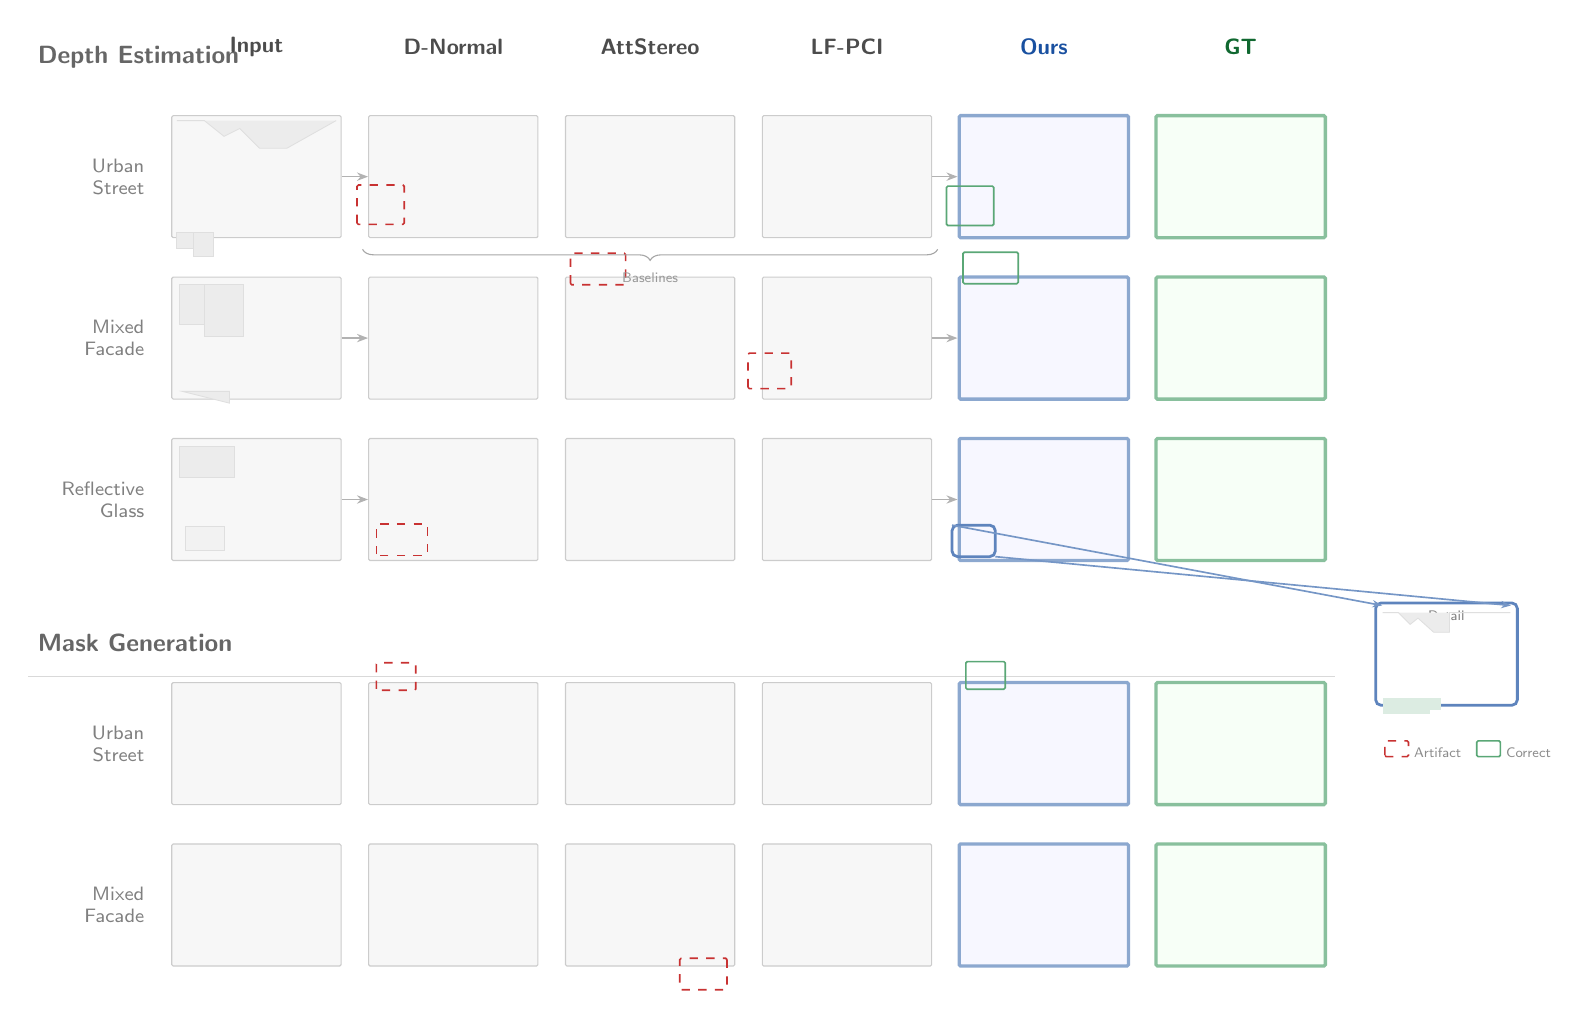
\begin{tikzpicture}[
  img/.style={
    draw=gray!40, minimum width=2.15cm, minimum height=1.55cm,
    fill=gray!6, inner sep=0pt, line width=0.4pt, rounded corners=0.5pt
  },
  imgo/.style={
    img, draw=oursblue!50, line width=1.2pt, fill=blue!3
  },
  imgg/.style={
    img, draw=gtgreen!50, line width=1.2pt, fill=green!3
  },
  hdr/.style={
    font=\sffamily\footnotesize\bfseries, text=black!70
  },
  rlbl/.style={
    font=\sffamily\scriptsize, text=black!50, align=right
  },
  stitle/.style={
    font=\sffamily\small\bfseries, text=black!60
  },
  errmark/.style={
    draw=errred, dashed, line width=0.6pt, rounded corners=0.5pt
  },
  goodmark/.style={
    draw=gtgreen!70, line width=0.6pt, rounded corners=0.5pt
  },
  zoombox/.style={
    draw=oursblue!70, line width=1pt, rounded corners=2pt
  },
  flowarr/.style={
    -{Stealth[length=4pt]}, semithick, color=black!30
  },
  zoomarr/.style={
    -{Stealth[length=3.5pt]}, semithick, color=oursblue!60
  },
  sceneicon/.style={
    draw=gray!25, line width=0.3pt, fill=gray!15
  }
]

% Layout parameters
\def\dx{2.5}
\def\dybase{-1.1}
\def\dystep{-2.05}

% ======== SECTION: Depth Estimation ========
\node[stitle, anchor=south west] at (-2.9, 0.15) {Depth Estimation};

% Column headers
\node[hdr] at (0*\dx, 0.55) {Input};
\node[hdr] at (1*\dx, 0.55) {D-Normal};
\node[hdr] at (2*\dx, 0.55) {AttStereo};
\node[hdr] at (3*\dx, 0.55) {LF-PCI};
\node[hdr, text=oursblue] at (4*\dx, 0.55) {Ours};
\node[hdr, text=gtgreen!80!black] at (5*\dx, 0.55) {GT};

% Row labels
\node[rlbl, anchor=east] at (-1.3, \dybase+0*\dystep) {Urban\\Street};
\node[rlbl, anchor=east] at (-1.3, \dybase+1*\dystep) {Mixed\\Facade};
\node[rlbl, anchor=east] at (-1.3, \dybase+2*\dystep) {Reflective\\Glass};

% ---- Row 1: Urban Street ----
\node[img] (r1c1) at (0*\dx, \dybase+0*\dystep) {};
\node[img] (r1c2) at (1*\dx, \dybase+0*\dystep) {};
\node[img] (r1c3) at (2*\dx, \dybase+0*\dystep) {};
\node[img] (r1c4) at (3*\dx, \dybase+0*\dystep) {};
\node[imgo] (r1c5) at (4*\dx, \dybase+0*\dystep) {};
\node[imgg] (r1c6) at (5*\dx, \dybase+0*\dystep) {};

% Scene icon in input
\draw[sceneicon] ([shift={(2pt,-2pt)}]r1c1.north west) -- ++(0.35,0) -- ++(0.25,-0.2) -- ++(0.2,0.1) -- ++(0.25,-0.25) -- ++(0.35,0) -- ([shift={(-2pt,-2pt)}]r1c1.north east);
\draw[sceneicon] ([shift={(2pt,2pt)}]r1c1.south west) rectangle ++(0.3,-0.2);
\draw[sceneicon] ([shift={(8pt,2pt)}]r1c1.south west) rectangle ++(0.25,-0.3);

% ---- Row 2: Mixed Facade ----
\node[img] (r2c1) at (0*\dx, \dybase+1*\dystep) {};
\node[img] (r2c2) at (1*\dx, \dybase+1*\dystep) {};
\node[img] (r2c3) at (2*\dx, \dybase+1*\dystep) {};
\node[img] (r2c4) at (3*\dx, \dybase+1*\dystep) {};
\node[imgo] (r2c5) at (4*\dx, \dybase+1*\dystep) {};
\node[imgg] (r2c6) at (5*\dx, \dybase+1*\dystep) {};

% Scene icon in input row 2
\draw[sceneicon] ([shift={(3pt,-3pt)}]r2c1.north west) rectangle ++(0.4,-0.5);
\draw[sceneicon] ([shift={(12pt,-3pt)}]r2c1.north west) rectangle ++(0.5,-0.65);
\draw[sceneicon] ([shift={(4pt,3pt)}]r2c1.south west) -- ++(0.6,0) -- ++(0,-0.15) -- cycle;

% ---- Row 3: Reflective Glass ----
\node[img] (r3c1) at (0*\dx, \dybase+2*\dystep) {};
\node[img] (r3c2) at (1*\dx, \dybase+2*\dystep) {};
\node[img] (r3c3) at (2*\dx, \dybase+2*\dystep) {};
\node[img] (r3c4) at (3*\dx, \dybase+2*\dystep) {};
\node[imgo] (r3c5) at (4*\dx, \dybase+2*\dystep) {};
\node[imgg] (r3c6) at (5*\dx, \dybase+2*\dystep) {};

% Scene icon in input row 3
\draw[sceneicon] ([shift={(3pt,-3pt)}]r3c1.north west) rectangle ++(0.7,-0.4);
\draw[sceneicon, fill=gray!10] ([shift={(5pt,4pt)}]r3c1.south west) rectangle ++(0.5,0.3);

% ======== Error indicators on baseline methods ========
% Red dashed box around artifact region in D-Normal, row 1
\draw[errmark] ([shift={(-4pt,5pt)}]r1c2.south west) rectangle ++(0.6,0.5);

% Red dashed box in AttStereo, row 2
\draw[errmark] ([shift={(2pt,-3pt)}]r2c3.north west) rectangle ++(0.7,0.4);

% Red dashed box in LF-PCI, row 2
\draw[errmark] ([shift={(-5pt,4pt)}]r2c4.south west) rectangle ++(0.55,0.45);

% Red dashed box in D-Normal, row 3
\draw[errmark] ([shift={(3pt,2pt)}]r3c2.south west) rectangle ++(0.65,0.4);

% ======== Good result indicators ========
% Green box on Ours, row 1 (detail region)
\draw[goodmark] ([shift={(-4pt,5pt)}]r1c5.south west) rectangle ++(0.6,0.5);

% Green box on Ours, row 2
\draw[goodmark] ([shift={(2pt,-3pt)}]r2c5.north west) rectangle ++(0.7,0.4);

% ======== Flow arrows between columns ========
\draw[flowarr] (r1c1.east) -- (r1c2.west);
\draw[flowarr] (r1c4.east) -- (r1c5.west);

\draw[flowarr] (r2c1.east) -- (r2c2.west);
\draw[flowarr] (r2c4.east) -- (r2c5.west);

\draw[flowarr] (r3c1.east) -- (r3c2.west);
\draw[flowarr] (r3c4.east) -- (r3c5.west);

% ======== Zoom-in detail panel for Row 3 ========
% Zoom source: small rectangle on r3c5 (Ours)
\coordinate (zoomsrc) at ([shift={(-2pt,2pt)}]r3c5.south west);
\draw[zoombox] (zoomsrc) rectangle ++(0.55,0.4);

% Zoom target: enlarged box below
\node[zoombox, fill=white, minimum width=1.8cm, minimum height=1.3cm,
      anchor=north west] (zoomtgt) at ([shift={(0.6,-0.5)}]r3c6.south east) {};
\node[font=\sffamily\tiny, text=black!50, anchor=north] at (zoomtgt.north) {Detail};

% Zoom arrows (connecting lines)
\draw[zoomarr] (zoomsrc) ++(0,0.4) -- ([shift={(0.1,-0.05)}]zoomtgt.north west);
\draw[zoomarr] (zoomsrc) ++(0.55,0) -- ([shift={(-0.1,-0.05)}]zoomtgt.north east);

% Small scene silhouette in zoom box
\draw[sceneicon] ([shift={(3pt,-4pt)}]zoomtgt.north west)
  -- ++(0.2,0) -- ++(0.15,-0.15) -- ++(0.1,0.08)
  -- ++(0.2,-0.18) -- ++(0.2,0) -- ++(0,0.25)
  -- ([shift={(-3pt,-4pt)}]zoomtgt.north east);
\fill[gtgreen!15] ([shift={(3pt,3pt)}]zoomtgt.south west) rectangle ++(0.6,-0.2);
\fill[gtgreen!15] ([shift={(10pt,3pt)}]zoomtgt.south west) rectangle ++(0.5,-0.15);

% ======== Separator and Mask section ========
\def\maskoff{\dybase+3*\dystep-0.5}

\draw[black!15, line width=0.3pt] (-2.9, \maskoff+0.3) -- (5*\dx+1.2, \maskoff+0.3);

\node[stitle, anchor=south west] at (-2.9, \maskoff+0.5) {Mask Generation};

% Mask row labels
\node[rlbl, anchor=east] at (-1.3, \maskoff-0.55) {Urban\\Street};
\node[rlbl, anchor=east] at (-1.3, \maskoff-0.55+\dystep) {Mixed\\Facade};

% ---- Mask Row 1 ----
\node[img] (m1c1) at (0*\dx, \maskoff-0.55) {};
\node[img] (m1c2) at (1*\dx, \maskoff-0.55) {};
\node[img] (m1c3) at (2*\dx, \maskoff-0.55) {};
\node[img] (m1c4) at (3*\dx, \maskoff-0.55) {};
\node[imgo] (m1c5) at (4*\dx, \maskoff-0.55) {};
\node[imgg] (m1c6) at (5*\dx, \maskoff-0.55) {};

% ---- Mask Row 2 ----
\node[img] (m2c1) at (0*\dx, \maskoff-0.55+\dystep) {};
\node[img] (m2c2) at (1*\dx, \maskoff-0.55+\dystep) {};
\node[img] (m2c3) at (2*\dx, \maskoff-0.55+\dystep) {};
\node[img] (m2c4) at (3*\dx, \maskoff-0.55+\dystep) {};
\node[imgo] (m2c5) at (4*\dx, \maskoff-0.55+\dystep) {};
\node[imgg] (m2c6) at (5*\dx, \maskoff-0.55+\dystep) {};

% Error indicator on mask baseline
\draw[errmark] ([shift={(3pt,-3pt)}]m1c2.north west) rectangle ++(0.5,0.35);
\draw[errmark] ([shift={(-3pt,3pt)}]m2c3.south east) rectangle ++(-0.6,-0.4);

% Good indicator on mask ours
\draw[goodmark] ([shift={(3pt,-3pt)}]m1c5.north west) rectangle ++(0.5,0.35);

% ======== Brace annotations ========
% Brace under baselines
\draw[decorate, decoration={brace, amplitude=4pt, mirror}, black!35, line width=0.4pt]
  ([shift={(-2pt,-4pt)}]r1c2.south west) -- ([shift={(2pt,-4pt)}]r1c4.south east)
  node[midway, below=5pt, font=\sffamily\tiny, text=black!40] {Baselines};

% ======== Legend ========
\node[anchor=north west, font=\sffamily\tiny, text=black!45, align=left]
  at ([shift={(0,-0.3)}]zoomtgt.south west) {%
    \tikz\draw[errmark] (0,0) rectangle (0.3,0.2); Artifact\quad
    \tikz\draw[goodmark] (0,0) rectangle (0.3,0.2); Correct%
  };

\end{tikzpicture}
\end{document}